\chapter{Visualização de Sinópticos SVG}\label{chap:chap3}

\section*{}

Este capítulo deve começar por fazer uma apresentação detalhada do
problema a resolver\footnote{Na introdução a apresentação do
  problema foi breve.} podendo mesmo, caso se justifique,
constituir-se um capítulo com essa finalidade.

Deve depois dedicar-se à apresentação da solução sem detalhes de
implementação. 
Dependendo do trabalho, pode ser uma descrição mais teórica, mais
``arquitetural'', etc.

\section{Secção Exemplo}

Neste capítulo apresentam-se exemplos de formatação de figuras e
tabelas, equações e referências cruzadas.

Apresenta-se de seguida um exemplo de equação, completamente fora do contexto:
\begin{eqnarray}
CIF_1: \hspace*{5mm}F_0^j(a) &=& \frac{1}{2\pi \iota} \oint_{\gamma} \frac{F_0^j(z)}{z - a} dz\\
CIF_2: \hspace*{5mm}F_1^j(a) &=& \frac{1}{2\pi \iota} \oint_{\gamma} \frac{F_0^j(x)}{x - a} dx \label{eq:cif}
\end{eqnarray}

Na Equação~\ref{eq:cif} lorem ipsum dolor sit amet, consectetuer
adipiscing elit. Suspendisse tincidunt viverra elit. Donec tempus
vulputate mauris. Donec arcu. Vestibulum condimentum porta
justo. Curabitur ornare tincidunt lacus. Curabitur ac massa vel ante
tincidunt placerat. Cras vehicula semper elit. Curabitur gravida, est
a elementum suscipit, est eros ullamcorper quam, sed cursus velit
velit tempor neque. Duis tempor condimentum ante.

Phasellus imperdiet, orci vel pretium sollicitudin, magna nunc
ullamcorper augue, non venenatis dui nunc quis massa. Pellentesque
dolor elit, dapibus venenatis, viverra ultricies, accumsan cursus,
orci. Aliquam erat volutpat. Mauris ornare tristique leo. Maecenas
eros. Curabitur velit nunc, tincidunt vitae, dictum posuere, pulvinar
nec, diam. In suscipit mauris a nunc. Pellentesque gravida. Morbi quam
lacus, pretium eget, tincidunt vulputate, interdum sed,
turpis. Curabitur quis est. Sed lectus lorem, congue vel, dignissim
laoreet, blandit a, nisi. Aenean nunc ligula, tincidunt eu, hendrerit
vel, suscipit non, erat. Aliquam gravida. Integer non pede. In laoreet
augue id leo. Mauris placerat. 

A arquitetura do visualizador assenta sobre os seguintes conceitos
basecite{kn:ZPMD97}: 

\begin{itemize}
\item \textbf{Componentes} --- Suspendisse auctor mattis augue \emph{push};
\item \textbf{Praesent} --- Sit amet sem maecenas eleifend facilisis leo;
\item \textbf{Pellentesque} --- Habitant morbi tristique senectus et netus.
\end{itemize}

\subsection{Exemplo de Figura}

É apresentado na Figura~\ref{fig:arch} %da página~\pageref{fig:arch}
um exemplo de figura flutuante.

\begin{figure}[t]
  \begin{center}
    \leavevmode
    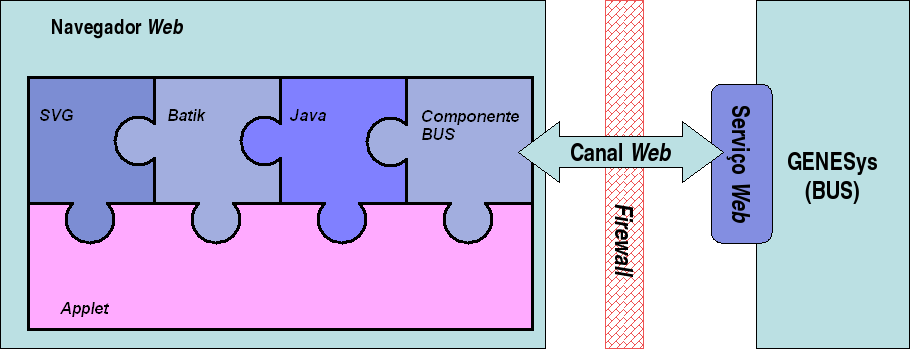
\includegraphics[width=0.86\textwidth]{puzzle}
    \caption{Arquitectura da Solução Proposta}
    \label{fig:arch}
  \end{center}
\end{figure}

Loren ipsum dolor sit amet, consectetuer adipiscing elit. 
Praesent sit amet sem. Maecenas eleifend facilisis leo. Vestibulum et
mi. Aliquam posuere, ante non tristique consectetuer, dui elit
scelerisque augue, eu vehicula nibh nisi ac est. Suspendisse elementum
sodales felis. Nullam laoreet fermentum urna. 

Duis eget diam. In est justo, tristique in, lacinia vel, feugiat eget,
quam. Pellentesque habitant morbi tristique senectus et netus et
malesuada fames ac turpis egestas. Fusce feugiat, elit ac placerat
fermentum, augue nisl ultricies eros, id fringilla enim sapien eu
felis. Vestibulum ante ipsum primis in faucibus orci luctus et
ultrices posuere cubilia Curae; Sed dolor mi, porttitor quis,
condimentum sed luctus. 

\subsection{Exemplo de Tabela}

É apresentado na Tabela~\ref{tab:exemplo1} um exemplo de tabela
flutuante e na Tabela~\ref{tab:exemplo2} um exemplo de tabela
flutuante, um pouco mais complicada.

\begin{table}[t]
  \centering
  \caption{Uma Tabela Simples}
\begin{tabular}{| l | p{45mm} |}
	\hline
\textbf{Acrónimo} & \textbf{Significado}\\
	\hline
	\hline
        ADT   & \emph{Abstract Data Type}\\\hline
        ANDF  & \emph{Architecture-Neutral Distribution Format}\\\hline
        API   & \emph{Application Programming Interface}\\
	\hline
\end{tabular}
  \label{tab:exemplo1}
\end{table}

Integer quis pede. Fusce nibh. Fusce nec erat vel mi condimentum
convallis. Sed at tortor non mauris pretium aliquet. In in lacus in
dolor molestie dapibus. Suspendisse potenti. Pellentesque sagittis
porta erat. Mauris sodales sapien id augue. Nam eu dolor. Donec sit
amet turpis non orci rhoncus commodo. Etiam condimentum commodo
libero.

Mauris pede. Curabitur faucibus dictum nibh. Proin tincidunt diam
vitae mauris. Sed hendrerit dolor vel ipsum. Nullam dapibus. Vivamus
tellus diam, egestas sit amet, vulputate non, vulputate id, eros. Nunc
sit amet nibh eget nibh imperdiet ornare. Cras vehicula mattis
ipsum. Sed diam arcu, semper at, gravida vitae, fermentum et,
nulla. Aenean massa orci, tristique nec, rutrum id, fringilla eget,
erat. Curabitur nulla ipsum, aliquam sed, rutrum vitae, semper quis,
ante. Fusce at nunc in dolor condimentum tempor. Duis sit amet massa. 

Curabitur convallis nulla quis risus. Nulla mollis porttitor
purus. Fusce ultricies odio at ligula pellentesque suscipit. Nulla
velit libero, blandit a, aliquet quis, hendrerit id, arcu. Phasellus
porttitor porttitor purus. Suspendisse velit tortor, fringilla sit
amet, commodo a, ultrices et, mi. Donec eu metus in erat ornare
adipiscing. Praesent varius mi ac nunc. Vestibulum leo lacus,
elementum in, vestibulum sit amet, hendrerit at, justo. Sed sit amet
neque. Donec libero risus, commodo sit amet, dignissim ut, tincidunt
a, eros. Ut non lacus quis tortor mattis ullamcorper. Vivamus
consequat augue vel erat. Sed tincidunt. Sed leo eros, ornare a,
pulvinar non, mattis quis, nibh. Aliquam faucibus mi ac nisi.

Pellentesque habitant morbi tristique senectus et netus et malesuada
fames ac turpis egestas. Duis aliquet, libero sit amet ornare viverra,
augue erat interdum dolor, vitae tincidunt lorem erat a lacus. Sed
lectus nisi, auctor in, hendrerit a, molestie vel, lectus. Cum sociis
natoque penatibus et magnis dis parturient montes, nascetur ridiculus
mus. Duis lacinia tempor dui. Vivamus rhoncus, tellus a viverra
dignissim, pede dui adipiscing odio, non faucibus metus mi gravida
eros. Nullam a tellus ut velit elementum tempus. Aenean rutrum
convallis tellus. Vestibulum nulla ante, dapibus ut, lobortis ut,
varius sed, nisl. Fusce lobortis. Sed ac lorem. Nulla tincidunt nulla
eget leo. Maecenas ac lectus eu neque ultrices pharetra. Curabitur a
risus nec arcu placerat tempor. Suspendisse magna nisl, viverra a,
adipiscing eget, ornare ultricies, ligula. Maecenas eu ligula vitae
eros convallis dignissim. 

\begin{table}[t]
  \centering
  \caption{Uma Tabela Mais Complicada}
\begin{tabular}{|c|r@{.}lr@{.}lr@{.}l||r|}
	\hline
\multicolumn{8}{|c|}
	{\rule[-3mm]{0mm}{8mm}Iteração $k$ de $f(x_n)$} \\
\textbf{\em k}
	& \multicolumn{2}{c}{$x_1^k$}
	& \multicolumn{2}{c}{$x_2^k$}
	& \multicolumn{2}{c||}{$x_3^k$}
	& comentários \\ \hline \hline
0   & -0&3                 & 0&6                 &  0&7   & - \\
1   &  0&47102965 & 0&04883157 & -0&53345964  & $\delta<\epsilon$ \\
2   &  0&49988691 & 0&00228830 & -0&52246185  & $\delta < \varepsilon$ \\
3   &  0&49999976 & 0&00005380 & -0&523656   &   $N$ \\
4   &  0&5                 & 0&00000307 & -0&52359743  & \\
\vdots	& \multicolumn{2}{c}{\vdots}
	& \multicolumn{2}{c}{$\ddots$}
	& \multicolumn{2}{c||}{\vdots}  & \\
7   &  0&5   & 0&0    & \textbf{-0}&\textbf{52359878}
		 & $\delta<10^{-8}$ \\ \hline
\end{tabular}
  \label{tab:exemplo2}
\end{table}

Loren ipsum dolor sit amet, consectetuer adipiscing elit. 
Praesent sit amet sem. Maecenas eleifend facilisis leo. Vestibulum et
mi. Aliquam posuere, ante non tristique consectetuer, dui elit
scelerisque augue, eu vehicula nibh nisi ac est. Suspendisse elementum
sodales felis. Nullam laoreet fermentum urna. 

Duis eget diam. In est justo, tristique in, lacinia vel, feugiat eget,
quam. Pellentesque habitant morbi tristique senectus et netus et
malesuada fames ac turpis egestas. Fusce feugiat, elit ac placerat
fermentum, augue nisl ultricies eros, id fringilla enim sapien eu
felis. Vestibulum ante ipsum primis in faucibus orci luctus et
ultrices posuere cubilia Curae; Sed dolor mi, porttitor quis,
condimentum sed luctus. 

\section{Secção Exemplo}

Loren ipsum dolor sit amet, consectetuer adipiscing elit. 
Praesent sit amet sem. Maecenas eleifend facilisis leo. Vestibulum et
mi. Aliquam posuere, ante non tristique consectetuer, dui elit
scelerisque augue, eu vehicula nibh nisi ac est. Suspendisse elementum
sodales felis. Nullam laoreet fermentum urna. 

Duis eget diam. In est justo, tristique in, lacinia vel, feugiat eget,
quam. Pellentesque habitant morbi tristique senectus et netus et
malesuada fames ac turpis egestas. Fusce feugiat, elit ac placerat
fermentum, augue nisl ultricies eros, id fringilla enim sapien eu
felis. Vestibulum ante ipsum primis in faucibus orci luctus et
ultrices posuere cubilia Curae; Sed dolor mi, porttitor quis,
condimentum sed luctus. 

\section{Resumo e Conclusões}

Resumir e apresentar as conclusões que se podem tirar no fim deste
capítulo.
